\chapter{COMPLEXITY ANALYSIS PLAN}\label{chap:complexity}

This chapter presents the expected time and space complexity of both algorithms and describes the methodology by which these bounds will be derived and empirically validated.

\section{Analytical Methodology}

The complexity of both algorithms will be analyzed using the standard \textbf{operation-counting} approach~\citep{cormen2009}:
\begin{enumerate}
    \item Identify all operations performed by the algorithm (heap insertions, extractions, edge relaxations, comparisons).
    \item Count the maximum number of times each operation is performed as a function of $|V|$ and $|E|$.
    \item Multiply by the cost of each operation (determined by the data structure) and sum to obtain the total complexity.
    \item Verify the asymptotic bound holds empirically by plotting runtime against $|V|$ and $|E|$ on log-log axes and checking that the slope matches the theoretical exponent.
\end{enumerate}

\section{Time Complexity}

\subsection{Baseline Dijkstra}

The time complexity analysis proceeds as follows~\citep{cormen2009,dijkstra1959}:

\begin{enumerate}
    \item \textbf{Initialization:} Setting \texttt{dist[v] = INF} and \texttt{parent[v] = NIL} for all $v \in V$ costs $O(|V|)$.
    \item \textbf{Priority queue insertions:} Each node is inserted at most once initially, and re-inserted (lazy) at most once per incoming edge. Total insertions $\leq |V| + |E|$. Each insertion costs $O(\log|V|)$ (binary heap sift-up). Total: $O(|E|\log|V|)$.
    \item \textbf{Extract-min operations:} Each node may be extracted multiple times (due to lazy insertion), but each extraction is $O(\log|V|)$. Total extractions $\leq |V| + |E|$. Total: $O(|E|\log|V|)$.
    \item \textbf{Edge relaxations:} For each extracted node $u$, all $\deg(u)$ outgoing edges are examined. Across the full algorithm, each edge is relaxed at most once: $\sum_{u\in V} \deg(u) = |E|$. Each relaxation costs $O(1)$ (comparison and hash map lookup). Total: $O(|E|)$.
\end{enumerate}

\noindent\textbf{Total time complexity:} $O(|E|\log|V|)$, dominated by heap operations~\citep{cormen2009}.

In sparse graphs where $|E| = O(|V|)$, this simplifies to $O(|V|\log|V|)$.

\textit{Note:} A Fibonacci heap would reduce the bound to $O(|E| + |V|\log|V|)$~\citep{fredman1987fibonacci}, but binary heaps are used here for practical simplicity and lower constant factors.

\subsection{Probability-Pruned Dijkstra}

\begin{enumerate}
    \item \textbf{Worst case ($\tau = 0$):} No edges are pruned; the algorithm is identical to the baseline. Worst-case time complexity: $O(|E|\log|V|)$.
    \item \textbf{Expected case ($\tau > 0$):} Let $|E'| \leq |E|$ denote the number of edges not pruned. Edges $(u,v)$ for which $\text{dist}[u] + w(u,v) > T$ are skipped in $O(1)$ without a heap insertion. The expected complexity is $O(|E'|\log|V|)$, where $|E'|$ depends on $\tau$ and the probability distribution.
    \item \textbf{Analysis of $|E'|$:} The fraction of edges pruned will be characterized empirically as a function of $\tau$, graph size $|V|$, and probability distribution (uniform vs.\ skewed). The expected pruning ratio $1 - |E'|/|E|$ will be plotted against $\tau$ to empirically characterize how aggressively each configuration benefits from pruning.
\end{enumerate}

\subsection{Empirical Validation Plan}

To verify that the theoretical bounds hold in practice, the following procedure will be followed:
\begin{itemize}
    \item For each graph size $|V| \in \{1{,}000,\;5{,}000,\;10{,}000,\;50{,}000\}$, measure mean execution time $T(|V|)$.
    \item Plot $\log T$ vs.\ $\log|V|$ (for sparse graphs where $|E| \propto |V|$) and verify slope $\approx 1$ (linear in $|V|\log|V|$).
    \item For the pruned algorithm, additionally plot $T_{\text{pruned}}$ vs.\ $|E'|/|E|$ to confirm that runtime scales proportionally to the fraction of edges explored.
\end{itemize}

\section{Space Complexity}

Both algorithms use the following data structures:

\begin{table}[h!]
\centering
\renewcommand{\arraystretch}{1.3}
\begin{tabular}{@{}lll@{}}
\toprule
\textbf{Data Structure} & \textbf{Space} & \textbf{Purpose} \\
\midrule
Adjacency list & $O(|V|+|E|)$ & Graph representation \\
Distance array \texttt{dist[v]} & $O(|V|)$ & Shortest path estimates \\
Parent array \texttt{parent[v]} & $O(|V|)$ & Path reconstruction \\
Priority queue (heap) & $O(|V|+|E|)$ worst case & Node ordering \\
\midrule
\textbf{Total} & $\mathbf{O(|V|+|E|)}$ & \\
\bottomrule
\end{tabular}
\caption[Space complexity breakdown]{Space complexity breakdown. Total is $O(|V|+|E|)$; in sparse graphs ($|E|=O(|V|)$) this reduces to $O(|V|)$ in practice.}
\label{table:space_complexity}
\end{table}

As shown in Table~\ref{table:space_complexity}, the dominant terms are the adjacency list and the priority queue, both $O(|V|+|E|)$. In the sparse graphs used in this project ($|E|=O(|V|)$), the total space simplifies to $O(|V|)$ in practice. Crucially, the pruning threshold $\tau$ adds no asymptotic space overhead: no additional arrays or data structures are required beyond those of the baseline algorithm.

\subsection{Empirical Memory Validation Plan}

Peak memory usage will be measured using Python's \texttt{tracemalloc} module across all input sizes. The expected behavior is:
\begin{itemize}
    \item Memory should grow approximately linearly with $|V|$ for sparse graphs (confirming $O(|V|)$ practical space).
    \item The pruned algorithm should exhibit lower peak priority queue memory due to fewer heap insertions, even though the asymptotic bound is the same.
    \item Memory results will be plotted against $|V|$ and compared to the theoretical $O(|V|+|E|)$ bound to confirm agreement.
\end{itemize}

\section{Summary of Expected Complexity}

Table~\ref{table:complexity_summary} summarises the time and space complexity for all three configurations.

\begin{table}[h!]
\centering
\renewcommand{\arraystretch}{1.4}
\begin{tabular}{@{}lccc@{}}
\toprule
\textbf{Algorithm} & \textbf{Time (worst)} & \textbf{Time (expected)} & \textbf{Space} \\
\midrule
Baseline Dijkstra & $O(|E|\log|V|)$ & $O(|E|\log|V|)$ & $O(|V|+|E|)$ \\
Pruned Dijkstra ($\tau=0$) & $O(|E|\log|V|)$ & $O(|E|\log|V|)$ & $O(|V|+|E|)$ \\
Pruned Dijkstra ($\tau>0$) & $O(|E|\log|V|)$ & $O(|E'|\log|V|)$, $|E'|\leq|E|$ & $O(|V|+|E|)$ \\
\bottomrule
\end{tabular}
\caption[Complexity summary]{Time and space complexity summary. Pruning reduces expected-case time to $O(|E'|\log|V|)$ with $|E'|\leq|E|$; worst-case and space bounds are unchanged.}
\label{table:complexity_summary}
\end{table}

When $\tau=0$ the pruned algorithm is identical to the baseline in all respects. For $\tau>0$, the worst-case bound is unchanged because in the worst case no path exceeds the threshold and all edges are processed. The practical benefit materialises in the expected case: edges whose accumulated log-cost exceeds $T=-\log(\tau)$ are skipped, reducing the effective edge count from $|E|$ to $|E'|\leq|E|$ and shrinking priority queue operations accordingly. These theoretical bounds will be validated empirically in Chapter~\ref{chap:results}.

Figure~\ref{fig:complexity_overview} summarises the full complexity and correctness properties of both algorithms in a side-by-side comparison, including the convergence guarantee and fallback strategy.

\begin{figure}[h!]
\centering
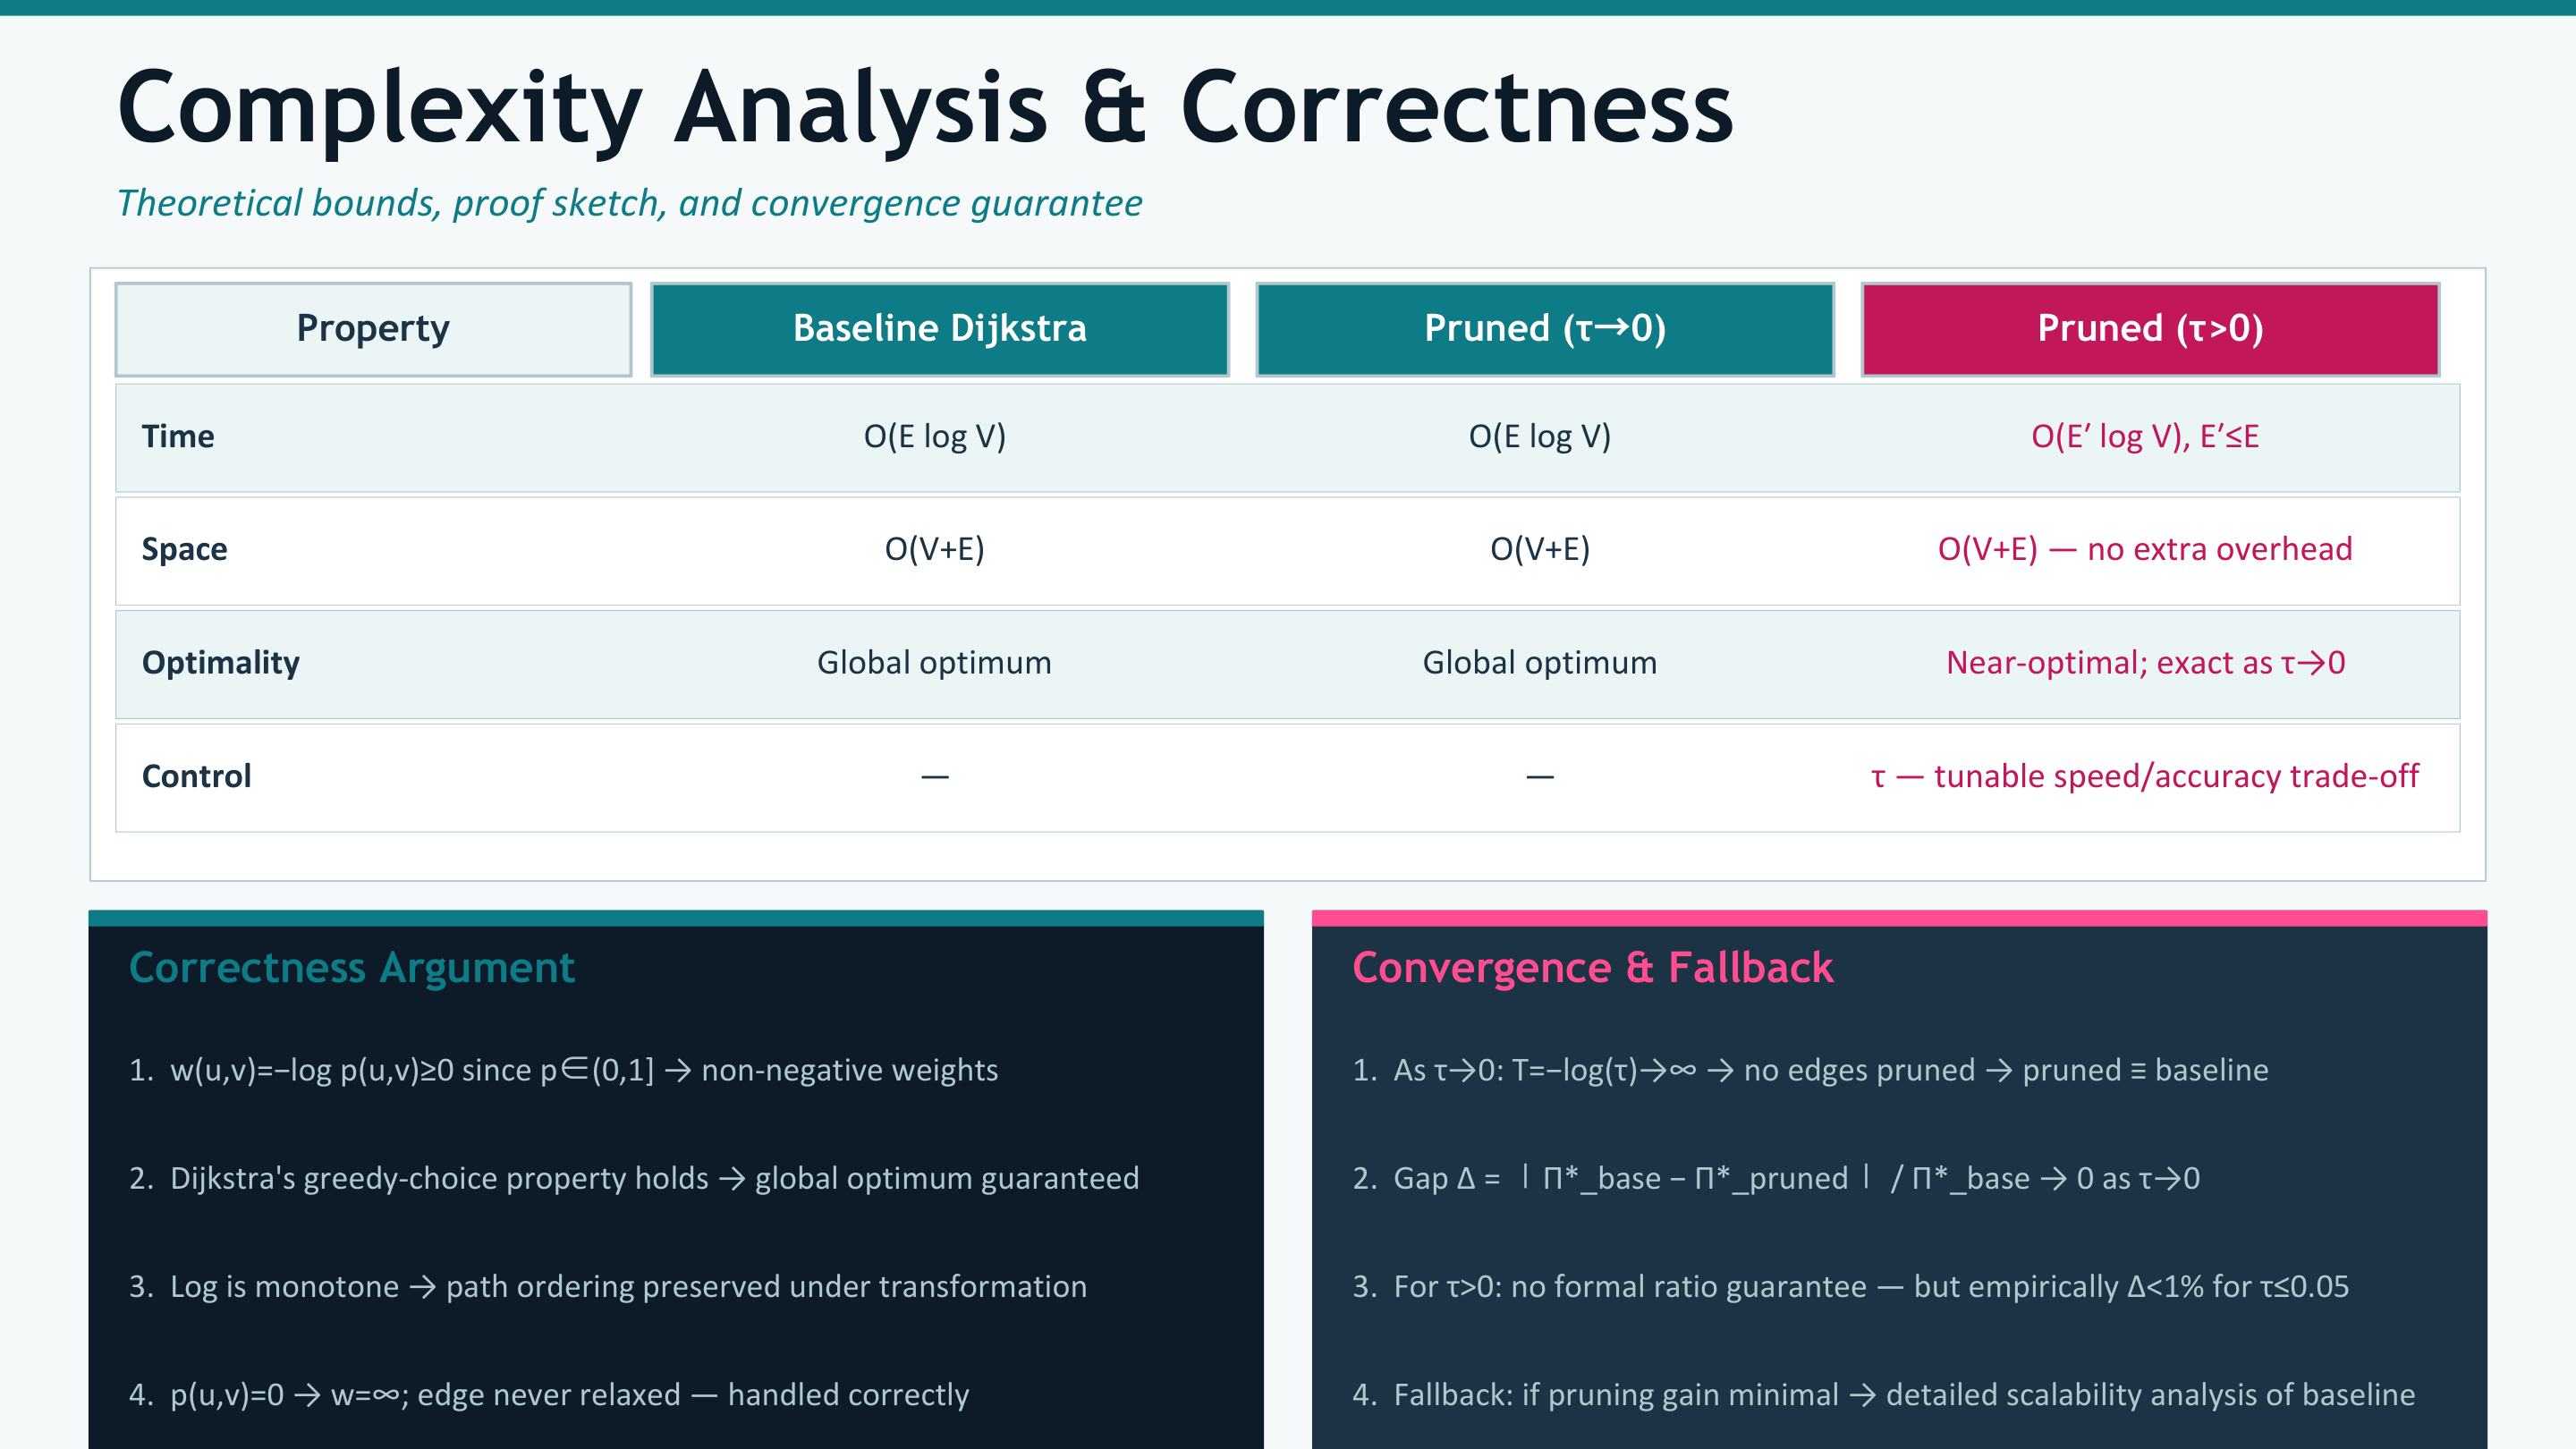
\includegraphics[width=0.95\textwidth]{complexity_table}
\caption[Complexity and correctness summary for both algorithms]{Summary of complexity and correctness properties. The upper table compares Time, Space, Optimality, and Control properties across three configurations (Baseline, Pruned $\tau\to0$, Pruned $\tau>0$). The lower panels give the four-point correctness argument (non-negative weights, greedy-choice invariant, monotone log-transform, zero-probability handling) and the four-point convergence guarantee ($\tau\to0$ recovers baseline; gap $\Delta\to0$; empirical $\Delta<1\%$ for $\tau\leq0.05$; fallback to baseline scalability analysis if pruning gain is minimal).}
\label{fig:complexity_overview}
\end{figure}
